\section{Utregning}

\subsection{Oppgave 1}
\subsubsection{Oppgave 5.1.21}
Prove the second-order formula for the fourth derivative
\begin{quote}
\begin{equation}\label{eq:oppgave1}
f^{(4)} (x) = \frac{f(x-2h) - 4f(x-h) + 6f(x) - 4f(x+h) + f(x+2h)}{h^4} + O(h^2)
\end{equation}
\end{quote}
Ifølge Taylor's teorem, dersom f er fem ganger kontinuerlig deriverbar, 
kan vi bruke f(x + h) og f(x -h)
\begin{quote}
\begin{equation} \label{eq:f(x+h)}
f(x+h) = f(x) + hf'(x) + \frac{h^2}{2} f''(x) + \frac{h^3}{6} f'''(x) + \frac{h^4}{24} f^4 (x) + \frac{h^5}{120} f^5 (x) + O(h^6)
\end{equation}
\end{quote}
\begin{quote}
\begin{equation} \label{eq:f(x-h)}
f(x-h) = f(x) - hf'(x) + \frac{h^2}{2} f''(x) - \frac{h^3}{6} f'''(x) + \frac{h^4}{24} f^4 (x) - \frac{h^5}{120} f^5 (x) + O(h^6)
\end{equation}
\end{quote}
Legger så sammen f(x+h) + f(x-h) for å eliminere odde-talls deriverte:

\begin{multline} \label{eq:f(x+h)+f(x-h)}
f(x+h) + f(x-h) = \\f(x) + hf'(x) + \frac{h^2}{2} f''(x) + \frac{h^3}{6} f'''(x) + \frac{h^4}{24} f^4 (x) + \frac{h^5}{120} f^5 (x) + O(h^6) +\\
 f(x) - hf'(x) + x\frac{h^2}{2} f''(x) - \frac{h^3}{6} f'''(x) + \frac{h^4}{24} f^4 (x) - \frac{h^5}{120} f^5 (x) + O(h^6) \\ = 2f(x) + h^2 f''(x) + \frac{h^4}{12} f^{(4)} (x) + O (h^6)
\end{multline}
I følge Taylor's teorem, dersom f er fem ganger kontinuerlig deriverbar, kan vi bruke f(x+2h) og f(x-2h). \\
Legger så sammen f(x+2h) + f(x-2h) for å eliminere oddetalls-deriverte. \\
Siden vi allerede har regnet ut f(x+h) + f(x-h), setter vi inn for f(x+2h) og f(x-2h) og får:
\begin{equation} \label{eq:f(x+2h)+f(x-2h)}
f(x+2h) + f(x-2h) = 2f(x) + 2h^2 f(x) + \frac{4h^4}{3} f^4 (x) + O (h^6)
\end{equation}
For å få den fjerde-deriverte aleine, må vi eliminere den andre-deriverte. Dette gjøres ved å gange inn 4 i den første likningen (\ref{eq:f(x+h)+f(x-h)}) og trekker fra likning (\ref{eq:f(x+2h)+f(x-2h)}): 

\begin{multline*}
4 * (f(x+h) + f(x-h)) = 8f(x) + 4h^2 f''(x) + \frac{4h^4}{12} f^4 + 4O(h^6) \\
\Downarrow
\\
4f(x+h) + 4f(x-h) - (f(x+2h) + f(x-2h)) = \\ 
8f(x) + 4h^2 f''(x) + \frac{4h^4}{12} f^4 (x) + 4O(h^6) - \\
2f(x) + 2h^2 f(x) + \frac{4h^4}{3} f^4 (x) + O (h^6) \\
= 6f(x) - h^4 f^4 (x) + 3O (h^6)
\end{multline*}
Snur litt om på likningen og får at:
\begin{multline}
h^4 f^4 = -4f(x+h) - 4f(x-h) + f(x-2h) + f(x-2h) + 6f(x) + 3O(h^6)\\
\Rightarrow f^4 (x) = \frac{f(x-2h) - 4f(x-h) + 6f(x) - 4f(x+h) + f(x+2h)}{h^4} + O(h^2)
\end{multline}


\subsubsection{Oppgave 5.1.22a}
Prove that if f(x) = f'(x) = 0, then
\begin{quote}
\begin{equation}\label{eq:oppgave2}
f^{(4)} (x + h) - \frac{16f(x + h) - 9f(x + 2h) + \frac{8}{3}f(x + 3h) - \frac{1}{4}f(x + 4h)}{h^4} = O(h^2)
\end{equation}
\end{quote}
Starter med å bevise at dersom f(x) = f'(x) = 0, så er
\begin{quote}
\begin{equation}
f(x + h) - 10f(x+h) + 5f(x + 2h) - \frac{5}{3}f(x + 3h) - \frac{1}{4}(x+4h) = O(h^6)
\end{equation}
\end{quote}
Fra oppgave 1, 5.1.21 har vi (\ref{eq:oppgave1}), vi begynner med å skrive denne om til f(x+h) og får:
\begin{quote}
\begin{equation}\label{eq:f^4(x+h)}
f^{(4)}(x+h) = \frac{-4f(x) + f(x-h) + 6f(x+h) - 4f(x+2h) f(x+3h}{h^4} + O(h^2)
\end{equation}
\end{quote}

Nå har vi en likning for $ f^{(4)} (x+h)$ og kan sette denne inn i (\ref{eq:oppgave2})


\begin{multline*}
\frac{-4f(x) + f(x-h) + 6f(x+h) - 4f(x+2h) + f(x+3h)}{h^4} + O(h^2)\\
-
\\
\frac{16f(x+h) - 4f(x+2h) + \frac{8}{3}f(x+3h) - \frac{1}{4}f(x+4h)}{h^4}  = O(h^2)
\\
\Downarrow
\\
\frac{-4f(x)+f(x-h)-10f(x+h)+5f(x+2h)-\frac{5}{3}f(x+3h)+\frac{1}{4}f(x+4h}{h^4} + O(h^2) = O(h^2)
\end{multline*}
Fra oppgaveteksten har vi oppgitt at:
\begin{equation*}
f(x-h)-10f(x+h)+5f(x+2h)-\frac{5}{3}f(x+3h)+\frac{1}{4}f(x+4h) = O(h^6)
\end{equation*}

Vi setter dette inn i likninger vår og får:

\begin{equation*}
\frac{-4f(x) + O(h^6)}{h^4} + O(h^2) = O(h^2)
\end{equation*}

Siden f(x) = f'(x) = 0 ender vi med:


\begin{equation*}
\frac{-0+ O(h^6)}{h^4} + O(h^2) = O(h^2)
\end{equation*}
\begin{equation*}
\Downarrow
\end{equation*}
\begin{equation*}
O(h^2) + O(h^2) = O(h^2)
\end{equation*}

\subsection{Oppgave 2}

lagA.m
\begin{lstlisting}
function A = lagA(n)

e = ones(n,1);
A = spdiags(e*[1 -4 6 -4 1],-2:2,n,n);

A(1,1:4) = [16 -9 8/3 -1/4];
A(n-1,n-3:n) = [16/17 -60/17 72/17 -28/17];
A(n,n-3:n)= [-12/17 96/17 -156/17 72/17];

end
\end{lstlisting}

Scriptet for å kjøre koden:
\begin{lstlisting}
disp('Oppave 2')

A = lagA(10);
full(A)
\end{lstlisting}

\subsection{Oppgave 3}

ebbeam.m
\\
Kan sende med A i fra forrige oppgave, men velger å lage A på nytt slik at dette kan kjøres som et eget skript.
\begin{lstlisting}
% Input:
% E = young's modulus for a meterial
% L = length
% d = diameter
% g = gravity
% w = width
% D = density
function y = ebbeam(E,L,d,D,w,n)

I = w*d^3/12;
h = L/n;
g = 9.81;
b = repmat(-D*w*d*g , n,1) * h^4/(E*I);

A = lagA(n);

y = A\b;
end
\end{lstlisting}
Scriptet for å kjøre koden:
\begin{lstlisting}
disp('Oppgave 3')
format long;
E = 1.3e10;
D = 480;
w = 0.3;
L = 2;
d = 0.03;
n = 10;

disp('Numerisk losning')
y = ebbeam(E,L,d,D,w,n)
\end{lstlisting}

\subsection{Oppgave 4}
\subsubsection{Oppgave 4a}
Vi har at Euler-Bernouillilikningen,
\begin{quote}
\begin{equation}
EIy'''' = f(x)
\end{equation}
\end{quote}
er oppfylt av y(x), som er den vertikale forskyvningen av en L meter lang bjelke. Den korrekte løsningen av likningen med konstanten f(x) = f er;
\begin{quote}
\begin{equation}\label{eq:oppgave4}
y(x)=(f/24EI) x^2 (x^2-4Lx+6L^2)
\end{equation}
\end{quote}
Skal nå vise at y(x) er den korrekte løsningen ved å derivere den fire ganger og sette inn i Euler-Bernouillilikningen. Begynner med å finne den deriverte med hensyn på x. Vi behandler f/EI og L som konstanter.

Begynner med å finne den deriverte:
\begin{quote}
\begin{equation*}
y=(f/24EI)(x^4-4Lx^3+6L^2x^2)=
\end{equation*}
\begin{equation*}
y'=\frac{d}{dx}[(f/24EI)]\frac{d}{dx}[x^4-4Lx^3+6L^2x^2]=
\end{equation*}
\begin{equation*}
y'=(f/24EI)(4x^3-12Lx^2+12L^2x)=
\end{equation*}
\end{quote}
Her er den derivert en gang, fortsetter med å finne den andrederiverte:
\begin{quote}
\begin{equation*}
y''=\frac{d}{dx}[(f/24EI)]\frac{d}{dx}[4x^3-12Lx^2+12L^2x]=
\end{equation*}
\begin{equation*}
y''=(f/24EI)(12x^2-24Lx+12L^2)=
\end{equation*}
\end{quote}
Her har vi funnet den andrederiverte, fortsetter med å finne den tredjederiverte;
\begin{quote}
\begin{equation*}
y'''=\frac{d}{dx}[(f/24EI)]\frac{d}{dx}[12x^2-24Lx+12L^2]=
\end{equation*}
\begin{equation*}
y'''=(f/24EI)(24x-24L+0)=
\end{equation*}
\end{quote}
Her har vi funnet den tredjederiverte, fortsetter med å finne den fjerdederiverte;
\begin{quote}
\begin{equation*}
y''''=\frac{d}{dx}[(f/24EI)]\frac{d}{dx}[24x-24L]=
\end{equation*}
\begin{equation*}
y''''=(f/24EI)(24)=
\end{equation*}
\begin{equation*}
y''''=\frac{24f}{24EI}
\end{equation*}
\begin{equation*}
y''''=\frac{f}{EI}
\end{equation*}
\end{quote}
Vi har nå funnet den fjerdederiverte til y(x). Vi kan nå sette inn i Euler-Bernouillilikningen;
\begin{quote}
\begin{equation*}
(1) y'''' = \frac{f(x)}{EI}
\end{equation*}
\begin{equation*}
(2) EIy'''' = f(x)
\end{equation*}
\end{quote}
Setter likning (1) inn i likning (2)
\begin{quote}
\begin{equation*}
EI*\frac{f(x)}{EI} = f(x)
\end{equation*}
\begin{equation*}
f(x) = f(x)
\end{equation*}
\end{quote}
Her har vi vist at y(x) oppfyller likningen ved å derivere fire ganger.

\subsubsection{Oppgave 4b}
Skal vise at for den korrekte løsningen er $y^{(6)}$(c) = 0. Vi vet fra oppgave 4a at den 4. deriverte av den korrekte løsningen er:
\begin{equation*}
y^{(4)}(x) = \frac{f}{EI}
\end{equation*}
Vi kan derfra visa at den 6. deriverte er 0.
\begin{equation}
f^{(5)}(x) = \frac{d}{dx}[\frac{f}{EI}] = 0
\end{equation}
Deriverer m.h.p x og $\frac{f}{EI}$ er en konstant.
\begin{equation}
y^{(6)}(x) = \frac{d}{dx}[0] = 0
\end{equation}
Slik har vi vist at $y^{(6)}(c) = 0$.

\subsubsection{Oppgave 4c}
Bruker her MATLAB til å regne ut den korrekte løsningen $y_e = [y(0.2) y(0.4) y(0.6) ... y(2.0)]$ 
\begin{lstlisting}
disp('Oppgave 4c')
[E, I, D, d, w, f, g, L] = hentKonstanter();

% Regner ut den eksakte losningen ye.
ye = zeros(1,10);
count = 1;
for i = (0.2:0.2:2)
    ye(count) = correct_y(f,E,I,L,i);
    count = count + 1;
end
ye = transpose(ye)


% Lager samme A som oppgave 2 og regner ut A*ye.
disp('Regner ut C = Ay (A-matrisen er laget med lagA(10) fra oppgave 2)')
A = lagA(10);
C = A*ye
\end{lstlisting}
\subsubsection{Oppgave 4d}
Her skal vi sammenligne svaret fra oppgave 4c med vektoren $b$ fra oppgave 3 og finne foroverfeil og relativ foroverfeil til $Diff_4(y)= Ay$. Etterpå skal vi anta at relativ bakoverfeil er $\epsilon_{mach} = 2^{-52}$, finne feilforstørrelsen og sammenligne den med kondisjonstallet til $A$. Her er MATLAB-koden:
\begin{lstlisting}
disp('Oppgave 4d')
disp('Sammenligner svaret C fra c) med vektoren b fra oppgave 3')

% Gjenskaper vektoren b fra oppgave 3.
h = L/10;
b = repmat(f, 10, 1) * h^4/(E*I);
table(C, b)

% Finner foroverfeil FE ved aa ta ||C - b||
disp('foroverfeil:')
FE = max( abs(C-b) )

% Finner relativ foroverfeil rFE ved aa ta ||C - b|| / ||C||
disp('Relativ foroverfeil:')
rFE = (FE)/( max( abs(C) ) )

% Antar at relativ bakoverfeil er rBE=2^-52 og regner ut
% feilforstorrelsen som rFE/rBE, sammenligner med kondisjonstallet til A.
disp('Feilforstorrelse:')
rBE = 2^-52;
rFE/rBE
disp('Kondisjonstall til A:')
cond(full(A))
\end{lstlisting}
Resultatet av koden blir som følger:
\begin{lstlisting}
Oppgave 4d
Sammenligner svaret C fra c) med vektoren b fra oppgave 3

ans = 

              C                        b          
    _____________________    _____________________

    -7.72726153846148e-06    -7.72726153846154e-06
    -7.72726153846224e-06    -7.72726153846154e-06
    -7.72726153845833e-06    -7.72726153846154e-06
    -7.72726153846787e-06    -7.72726153846154e-06
    -7.72726153845486e-06    -7.72726153846154e-06
    -7.72726153846354e-06    -7.72726153846154e-06
    -7.72726153846007e-06    -7.72726153846154e-06
    -7.72726153846527e-06    -7.72726153846154e-06
    -7.72726153846354e-06    -7.72726153846154e-06
    -7.72726153846354e-06    -7.72726153846154e-06

foroverfeil:

FE =

     6.678007756152904e-18

Relativ foroverfeil:

rFE =

     8.642140197932253e-13

Feilforstorrelse:

ans =

     3.892073937509128e+03
     

Kondisjonstall til A:

ans =

     1.857401842242595e+04
\end{lstlisting}
Vi vet fra teorien at kondisjonstallet til A er den maksimale feilforstørrelsen man kan oppnå. Med et kondisjonstall på $10^4$ kan man forvente $16-4=12$ korrekte desimaler i svaret. ******* SKRIV MER **********

\subsubsection{Oppgave 4e}
Her skal vi sammenligne svaret fra oppgave 3, $y_c$, med den korrekte løsningen, $y_e$, fra oppgave 4c. Vi skal finne foroverfeilen $||y_c-y_e||_1$. Dette er en 1-norm som regnes ut som summen av absolutt-verdien til alle elementene i vektoren. Her er MATLAB-koden:
\begin{lstlisting}
disp('Oppgave 4e')
disp('Sammenligner den eksakte losningen (ye) med vektoren (yc) fra opgave 3')

yc = ebbeam(L,10,f,E,I);
table(yc, ye)

disp('foroverfeil: ||yc-ye||_1')
% Denne foroverfeilen er en 1-norm, kan regnes paa to maater:
sum(abs(yc-ye));
norm(yc-ye, 1)
\end{lstlisting}
Her er resultatet av koden:
\begin{lstlisting}
Oppgave 4e
Sammenligner den eksakte losningen (ye) med vektoren (yc) fra oppgave 3

ans = 

             yc                       ye          
    _____________________    _____________________

    -1.80624738461544e-04    -1.80624738461539e-04
    -6.74847507692328e-04    -6.74847507692308e-04
    -1.41698658461543e-03    -1.41698658461539e-03
    -2.34908750769237e-03    -2.34908750769231e-03
    -3.42092307692317e-03    -3.42092307692308e-03
    -4.58999335384627e-03    -4.58999335384616e-03
    -5.82152566153860e-03    -5.82152566153846e-03
    -7.08847458461555e-03    -7.08847458461539e-03
    -8.37152196923095e-03    -8.37152196923077e-03
    -9.65907692307711e-03    -9.65907692307692e-03

foroverfeil: ||yc-ye||_1

ans =

     9.980623098815311e-16
\end{lstlisting}
Vi ser at denne foroverfeilen er i samme størrelsesorden som $\epsilon_{mach}$, ******* HVORFOR? **********

\subsection{Oppgave 5}
Vi starter her med å hente inn konstantene vi fikk oppgitt i boken, deretter har vi definert at $n=10(2^{i})$ som oppgitt i oppgaven og bruker ebbeam-funksjonen som er 
Euler-Bernoulli sin metode for å beregne hvor mye materialet bøyer seg under press. 
Vi beregner den numeriske løsningen ved hjelp av ebbeam-funksjonen, den faktiske løsningen, feilen og kondisjonstallet. 
\begin{lstlisting}
format long;
[E, I, D, d, w, f, g, L, p] = hentKonstanter();
n = 10;

i_max = 11;

n = zeros(i_max, 1);
y_num_L = zeros(i_max, 1);
y_actual_L = zeros(i_max, 1);
error = zeros(i_max,1);
cond_A = zeros(i_max,1);

syms y(x) y(z);
y(x) = correct_y(f,E,I,L,x);

for i = (1:i_max)
    n(i) = 10*2^i;
    y_num = ebbeam(L,n(i),f,E,I);
    y_num_L(i) = y_num(n(i));
    y_actual_L(i) = y(L);
    error(i) = abs(y_actual_L(i) - y_num(n(i)));
    A = lagA(n(i));
    cond_A(i) = condest(A);
end

T = table(n, y_num_L, y_actual_L, error, cond_A);
disp(T);
figure;
plot(log(n), log(error));
hold on;
plot(log(n), log(cond_A));
title('Error figure and Condition Number - Oppgave 5');
\end{lstlisting}

\begin{lstlisting}
% Input:
% E = young's modulus for a meterial
% L = length
% d = diameter
% g = gravity
% w = width
% D = density
function y = ebbeam(L,n,f,E,I)

h = L/n;

%legg til sinusformel
b = repmat(f, n, 1) * h^4/(E*I);

A = lagA(n);
y = A\b;

end
\end{lstlisting}
Her er ebbeam-funksjonen.

\begin{lstlisting}
function y = correct_y(f, E, I, L, x)
    y = (f/(24*E*I))*x^2*(x^2 - 4*L*x + 6*L^2);
end
\end{lstlisting}
Dette er funksjonen for den korrekte løsningen, samme som i oppgave 4 (\ref{eq:oppgave4})

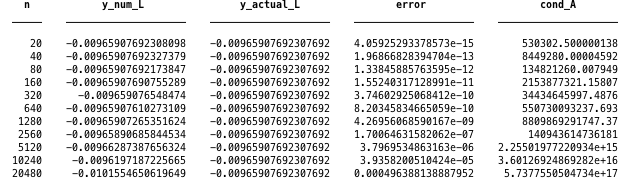
\includegraphics[width=\textwidth]{Oppgave5}
Ut i fra resultatet over er det lett å se hvilken n-verdi som gir størst feil, når n = 20. Man ser også at når n øker så minker feilen, dette er fordi jo flere intervaller vi har jo mer nøyaktig blir estimeringen. Vi ser også ut i fra resultatet at kondisjonstallet stiger lineært når n øker. \\
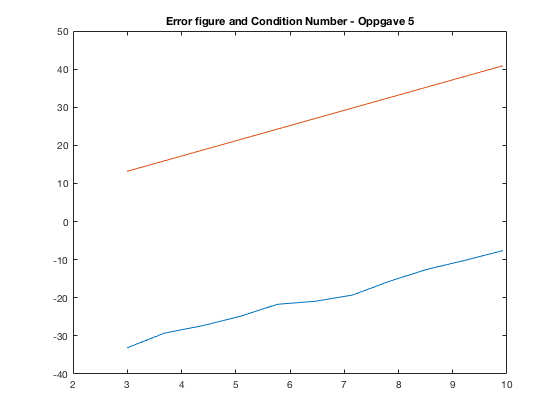
\includegraphics[width=\textwidth]{Oppgave5fig}
Grafen viser kondisjonstallet i en rett linje (rød), mens den blå linjen er feilen. Vi ser at når n øker, minsker feilen mens kondisjonstallet forsetter å øke.

\subsection{Oppgave 6}
\subsubsection{Oppgave 6a}
Vi legger til en funksjon i Euler-likningen
\begin{quote}
\begin{equation} \label{eq:sin(x)}
s(x) = -pgsin\frac{\pi}{L} x
\end{equation}
\end{quote} 
til kraftdelen til f(x)
\begin{quote}
$EIy^{(4)} = f(x) + s(x)$
\end{quote}
Skal bevise at
\begin{quote}
\begin{equation}\label{eq:oppgave6a}
y(x) = \frac{f}{24EI} x^2 (x^2 - 4Lx + 6L^2) - \frac{gpL}{EI\pi} (\frac{L^3}{\pi^3} sin\frac{\pi}{L}x - \frac{x^3}{6} + \frac{Lx^2}{2} - \frac{L^2 x}{\pi^2})
\end{equation}
\end{quote}
tilfredstiller Euler-Bernoullie likningen og randbetingelsene for en bjelke som er fast i den ene enden og fri i den andre\\
$y(0) = y'(0) = y''(L) = y'''(L) = 0$ \\
\\
1. Starter med å bevise at y(0)= 0
\begin{quote}
\begin{multline*}
y(0) = \frac{f}{24EI} 0^2 (0^2 - 4L0 + 6L^2) - \frac{gpL}{EI\pi} (\frac{L^3}{\pi^3} sin\frac{\pi}{L}x - \frac{0^3}{6} + \frac{L0^2}{2} - \frac{L^2 0}{\pi^2}) \\
y(0) = 0 - \frac{gpL}{EI\pi} (\frac{L^3}{\pi^3} sin (0) - 0 + 0 - 0 ) \\
y(0) = 0
\end{multline*}
\end{quote}
Første kriterie er oppfylt.
\\
2. Skal nå bevise kriterie 2, at y'(0) = 0, starter med å finne den deriverte.
\begin{quote}
\begin{multline}
y'(x) = \frac{d}{dx} [\frac{fx^2(x^2-4Lx+6L^2)}{24EI} - \frac{gpL}{EI\pi} (\frac{L^3}{\pi^3} sin \frac{\pi}{L}x - \frac{x^3}{6} + \frac{Lx^2}{2} - \frac{L^2x}{\pi^2})]
\end{multline}
\end{quote}

\begin{quote}
\begin{multline*}
y'(x) = \frac{fx(x^2-3Lx+3L^2)}{6EI} - \frac{gpL}{EI\pi}*\frac{d}{dx} (\frac{L^3}{\pi^3} sin \frac{\pi}{L}x - \frac{x^3}{6} + \frac{Lx^2}{2} - \frac{L^2x}{\pi^2})
\end{multline*}
\end{quote}

\begin{quote}
\begin{multline*}
y'(x) = \frac{fx(x^2-3Lx+3L^2)}{6EI} - \frac{gpL}{EI\pi} (\frac{L^2}{\pi^2} cos(\frac{\pi}{L}x) - \frac{x^2}{2} + Lx - \frac{L^2}{\pi^2})
\end{multline*}
\end{quote}
Sjekker om y'(0) = 0
\begin{quote}
\begin{multline*}
y'(0) = \frac{f0(0^2-3L0+3L^2)}{6EI} - \frac{gpL}{EI\pi} (\frac{L^2}{\pi^2} cos(\frac{\pi}{L}0) - \frac{0^2}{2} + L0 - \frac{L^2}{\pi^2})
\end{multline*}
\end{quote}

\begin{quote}
\begin{equation*}
y'(0) = 0 - \frac{gpL}{EI\pi} (\frac{L^2}{\pi^2} * 1 -\frac{L^2}{\pi^2}) \\
\end{equation*}
\end{quote}

\begin{quote}
\begin{equation*}
y'(0) = 0 - \frac{gpL}{EI\pi} (0) = 0
\end{equation*}
\end{quote}
Andre kriteriet er oppfylt.
\\
3. Skal nå bevise kriteriet 3, y''(L) = 0. Starter med å finne den andre deriverte.
\begin{quote}
\begin{multline*}
y'(x) = \frac{fx(x^2-3Lx+3L^2)}{6EI} - \frac{gpL}{EI\pi} (\frac{L^2}{\pi^2} cos(\frac{\pi}{L}x) - \frac{x^2}{2} + Lx - \frac{L^2}{\pi^2})
\end{multline*}
\end{quote}
Fra oppgave 4a, vet vi at
\begin{quote}
\begin{multline*}
y''(x) = \frac{f(x-L)^2}{2EI} - \frac{gpL}{EI\pi} \frac{d}{dx}(\frac{L^2}{\pi^2} cos(\frac{\pi}{L}x) - \frac{x^2}{2} + Lx - \frac{L^2}{\pi^2})
\end{multline*}
\end{quote}

\begin{quote}
\begin{multline}
y''(x) = \frac{f(x-L)^2}{2EI} - \frac{gpL}{EI\pi}* [\frac{L}{\pi} (-sin(\frac{\pi}{L}x)) - x + L]
\end{multline}
\end{quote}
Sjekker nå om y''(L)=0
\begin{quote}
\begin{multline}
y''(L) = \frac{f(L-L)^2}{2EI} - \frac{gpL}{EI\pi}* [\frac{L}{\pi} (-sin(\frac{\pi}{L}L)) - L + L]
\end{multline}
\end{quote}

\begin{quote}
\begin{equation*}
y''(L) = 0 - \frac{gpL}{EI\pi}* [\frac{L}{\pi} (-sin(\pi)) ]
\end{equation*}
\end{quote}

\begin{quote}
\begin{equation*}
y''(L) = 0 - \frac{gpL}{EI\pi}* [\frac{L}{\pi} (0) ]
\end{equation*}
\end{quote}

\begin{quote}
\begin{equation*}
y''(L) = 0 - 0 = 0
\end{equation*}
\end{quote}
Tredje kriteriet stemmer da y''(L) = 0.
4. Skal nå bevise at fjerde kriteriet, y'''(L) = 0, og starter med å finne den tredje deriverte
\begin{quote}
\begin{multline*}
y''(x) = \frac{f(x-L)^2}{2EI} - \frac{gpL}{EI\pi}(\frac{L^2}{\pi^2} cos(\frac{\pi}{L}x) - \frac{x^2}{2} + Lx - \frac{L^2}{\pi^2})
\end{multline*}
\end{quote}

\begin{quote}
\begin{multline*}
y'''(x) = \frac{f(x-L)^2}{2EI} - \frac{gpL}{EI\pi} \frac{d}{dx}(\frac{L^2}{\pi^2} cos(\frac{\pi}{L}x) - \frac{x^2}{2} + Lx - \frac{L^2}{\pi^2})
\end{multline*}
\end{quote}

\begin{quote}
\begin{equation}
y'''(x) = \frac{f(x-L)}{EI} - \frac{gpL}{EI\pi} (-cos(\frac{\pi}{L}x) - 1)
\end{equation}
\end{quote}
Sjekker så tredje kriteriet, y'''(L) = 0
\begin{quote}
\begin{equation*}
y'''(L) = \frac{f(L-L)}{EI} - \frac{gpL}{EI\pi} (-cos(\frac{\pi}{L}L) - 1)
\end{equation*}
\end{quote}

\begin{quote}
\begin{equation*}
y'''(L) = 0 - \frac{gpL}{EI\pi} (1 - 1)
\end{equation*}
\end{quote}

\begin{quote}
\begin{equation*}
y'''(L) = 0 - \frac{gpL}{EI\pi} 0 = 0
\end{equation*}
\end{quote}
Fjerde kriteriet stemmer fordi y'''(L) = 0.

\subsubsection{Oppgave 6b}
I denne oppgaven skal vi legge en sinusformet haug på stupebrettet og kjøre forløkka fra Oppgave 5 om igjen. Vi bruker den samme utformingen på oppgaven.

\begin{lstlisting}
format long;
[E, I, D, d, w, f, g, L, p] = hentKonstanter();

i_max = 11;

n = zeros(i_max, 1)
numeric = zeros(i_max, 1);
actual = zeros(i_max, 1);
error = zeros(i_max,1);
cond_A = zeros(i_max,1);

syms y(x) ;
y(x) = correct_y_sin(f, E, I, L, p, g, x);


for i = (1:i_max)
    n(i) = 10*2^i;
    y_num = ebbeam_s(L,n(i),f,E,I,p,g);
    numeric(i) = y_num(n(i));
    actual(i) = y(L);
    error(i) = abs(actual(i) - numeric(i));
    A = lagA(n(i));
    cond_A(i) = condest(A);
end

T = table(n, numeric, actual, error, cond_A);
disp(T);
figure;
subplot(2,1,1)
plot(numeric);
hold on;
plot(actual);
title('Actual vs numeric');
subplot(2,1,2);
loglog(n,error);
hold on;
plot(n,cond_A*eps, ':');
hold on;
h_sq = ((ones(i_max, 1))*(L^2)) ./ (n.^2);
disp(h_sq);
plot(n, h_sq, '--');
title('Error, Theoretical Error and Condition Number');
\end{lstlisting}
For å ta sinushaugen i betrakning trenger vi å endre på den korrekte- og den numeriske formelen. Vi legger sinuskraften i den korrekte formelen:
\\
\begin{lstlisting}
function y = correct_y_sin(f, E, I, L, p, g, x)
    y = ((f/(24*E*I))*x^2*(x^2 - 4*L*x + 6*L^2)) - (((p*g*L)/(E*I*pi))*(((L^3)/(pi^3))*sin(pi*x/L)-(x^3)/6+(L*x^2)/2-x*(L^2)/(pi^2)));
end
\end{lstlisting}

Denne kan se litt komplisert ut, men det er bare en omskriving av denne formelen fra Oppgave 6a (\ref{eq:oppgave6a})
\\Vi trenger også å skrive om den numeriske løsningen:

\begin{lstlisting}
function y = ebbeam_s(L,n,f,E,I,p,g)

h = L/n;

x = sin_x((h:h:L),p,g,L)';

b = repmat(f, n, 1);
b = b + x;
b = b * ((h^4/(E*I)));

A = lagA(n);
y = A\b;

end
\end{lstlisting}

Her legger vi til kraften fra sinushaugen ved å opprette en vektor x som kaller på sinus-funksjonen i en løkke n-antall ganger. Sinusfunksjonen ser ut som følger

\begin{lstlisting}
function y = sin_x(x, p, g, L)

y = (-p*g*(sin((pi/L)*x)));

end
\end{lstlisting}

Dette er sinuskraften fra Oppgave 6a (\ref{eq:sin(x)})
\\Dette produserer resultatet:

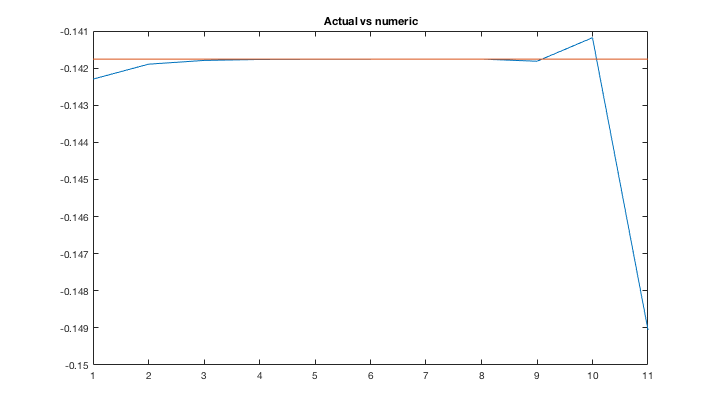
\includegraphics[width=\textwidth]{oppgave6b}
Vi ser her at den numeriske (blå) løsningen er ganske lik den korrekte løsningen. Vi ser også at når vi kommer over $10(2^{10})$ intervaller begynner resultatet å oppføre seg litt rart. I følge Taylorrekken skulle vi med flere iterasjoner få en mer nøyaktig løsning.

\subsubsection{Oppgave 6c, d, e og f}
Vi gjør som vi har gjort tidligere og regner ut feilmarginen og kondisjonstallet for A. Forskjellen i denne oppgaven er at vi ganger kondisjonstallet til a med $\epsilon_{mach}$ som er $2^{-52}$. Den teoretiske feilen $h^2 = L^2 / n^2$.Resultatet blir som følger:
\\
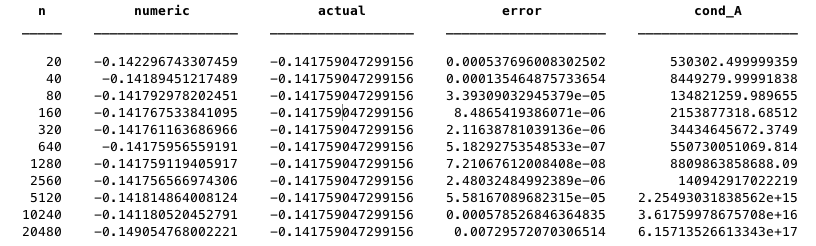
\includegraphics[width=\textwidth]{oppgave6numbers}
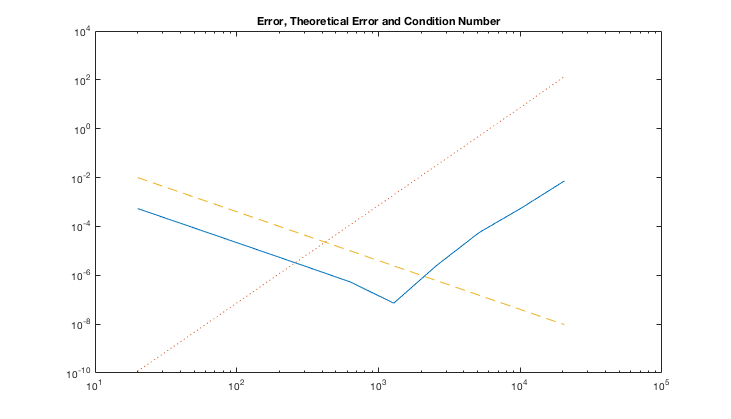
\includegraphics[width=\textwidth]{oppgave6cd}
Dette hadde vi ikke forventet. Vi skulle tro at jo flere iterasjoner vi hadde, jo mindre ble feilen. Vi ser også at den teoretiske feilen (gul) avtar med høyere n-verdi. Legg merke til at når feilen snur og begynner å bli større, følger den kondisjonstallet (rød). Vi konkluderer med at ved bunnpunktet blir kondisjonstallet dominerende, og feilen begynner å øke. Ut fra grafen ser vi også at den optimale verdien til n = $10(2^7) = 1280$.

\subsubsection{Oppgave 7}
I denne oppgaven skal vi bytte ut den sinusformede haugen med en person som veier 50kg og som står ytterst på stupebrettet. Vi antar at all vekten til personen er jevnt fordelt utover foten som er 30cm. Vi trenger å legge til kraft pr. enhetslengde definert ved: 

\[ s_{2}(x) =
  \begin{cases}
    (-9.81)(50kg)/0.3kg/m       & \quad L - 0.3m \leq x \leq L\\
    0N/m  & \quad 0m \leq x < L - 0.3m\\
  \end{cases}
\]

\begin{lstlisting}
format long;
[E, I, D, d, w, f, g, L, p] = hentKonstanter();
i_max = 11;

n = zeros(i_max, 1);
numeric = zeros(i_max, 1);
actual = zeros(i_max, 1);
error = zeros(i_max,1);
cond_A = zeros(i_max,1);

syms y(x);
y(x) = correct_y(f,E,I,L,x);

for i = (1:i_max)
    n(i) = 10*2^i;
    y_num = ebbeam_7(L,n(i),f,E,I,g);
    numeric(i) = y_num(n(i));
end

T = table(n, numeric);
figure;
plot(numeric);

disp(T);
\end{lstlisting}
Vi har i denne oppgaven valgt å lage en ny ebbeam-funksjon hvor vi fordeler kraften fra personen på stupebrettet.
\begin{lstlisting}
function y = ebbeam_7(L,n,f,E,I,g)

h = L/n;
b = zeros(n, 1);
load = -g*50 / 0.3;

for i = ceil(1.7/h):n
    b(i) = load;
end

b = b + repmat(f, n, 1);
b = b * ((h^4/(E*I)));

A = lagA(n);
y = A\b;

end
\end{lstlisting}
Vi begynner med å opprette b-vektoren som får størrelsen n og fylles med 0. "load" er kraften fra personen i Newton fordelt på hans 30cm. For å fordele kraften pr. enhetslengde bruker vi en finulig forløkke som legger til kraften på de ytterste 30cm av stupebrettet. Når vi kjører skriptet til Oppgaven får vi følgende resultat:
\begin{lstlisting}

      n           numeric      
    _____    __________________

       20    -0.161606940171006
       40    -0.151735608265121
       80    -0.146855330241007
      160    -0.144429229072343
      320    -0.143219706797572
      640    -0.142615828284291
     1280    -0.142314058185972
     2560     -0.14216085974436
     5120     -0.14214359762075
    10240    -0.141473578950692
    20480    -0.149305718176302
\end{lstlisting}
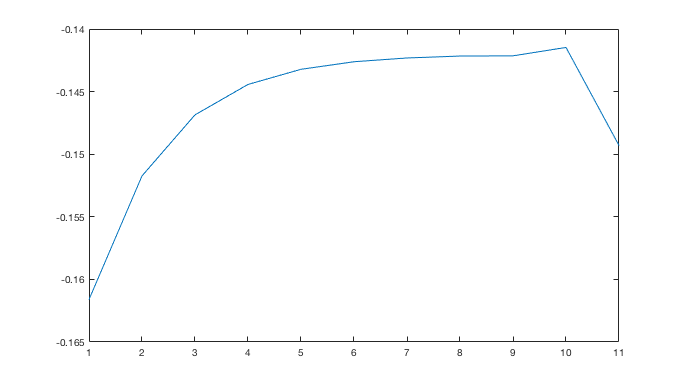
\includegraphics[width=\textwidth]{oppgave7}
Grafen viser hvor mye stupebrettet bøyer seg ytterst med forskjellige n-verdier. Ut fra resultatene kan vi se likheter fra oppgave 6. Vi begynner å få like resultater når n er større enn 160. Dette gir oss en trygghet om at svaret nærmer seg den korrekte løsningen. Denne trenden fortsetter frem til n blir større enn $10(2^10)$, da får vi et ulikt resultat, og til sist blir resultatet veldig forskjellig fra trenden. Vi vet at når kondisjonstallet øker, øker feilen i resultet gitt en liten feil i inn-dataen. Fra oppgave 6 vet vi også at kondisjonstallet øker lineært med antall intervaller, og her kan vi konkludere med at kondisjonstallet er så stort at vi får store feil i resultatet. Ut fra dette kan vi si at den beste verdien av n vil være lik den i oppgave 6, rundt $n = 10(2^7)$.